\documentclass{article}
\usepackage{style}
\usepackage{MyNotations}
\begin{document}


\section{Finite element implementation of the coupled model}
\subsection{Weak coupling under periodic boundary conditions}
\subsubsection{Swif-Hohenberg equation}
We recall that \textit{Swift-Hohenberg equation} is a non-linear fourth order partial differential equation, defined as :
\begin{equation}\label{eq:SH4th}
   \frac{\partial \psi}{\partial t} = - \Gamma \frac{\delta \mathcal{F}}{\delta \psi} = - \Gamma \left[ \psi + f'(\psi) + \Delta^2 \psi +2 \Delta \psi  \right] \quad \text{with} \quad f(\psi) = -\frac{\epsilon}{2} \psi^2 - \frac{g}{3}\psi^3 + \frac{1}{4} \psi^4
\end{equation}
Several numerical methods have been proposed in the literature, trying to build a thermodynamically consistent and energy stable schemes while optimizing the computational costs.
It is well known that a forward explicit euler scheme is unstable if the CFL-like conditions are not met $(\Delta t\sim < \Delta x^4)$. For this reason, a first semi-implicit method was proposed in \cite{chengEfficientAlgorithmSolving2008}, then this method was enhanced in \cite{elseySimpleEfficientScheme2013} where the authors added a stabilizing term to enforce energy stability. Following this, a second order Crank-Nicolson scheme was suggested in \cite{gomezNewSpaceTime2012} in combination with a Newton-Raphson method to adress the non linear scheme. Moreover, to deal with the non-linear term, different operator splitting methods were proposed, such as first and second order convex splitting \cite{huStableEfficientFinitedifference2009}. Finally, we refer to spectral method used in conjunction with these splitting methods (e.g \cite{leeSemianalyticalFourierSpectral2017}) and pseudo-spectral studied in \cite{zhaiStabilityErrorEstimate2021}.
In what comes next, we follow the finite elements scheme suggested in \cite{qiNumericalAnalysisSecondorder2024}, based on the classically used mixed formulation of fourth order partial differential equations. We argue that, the mixed formulation is the simplest way to solve fourth order PDEs weakly without the need to use high order $H^2$ elements, non-conformal and penalty methods. \marginpar{Add refs}\\

We consider a domain $\Omega$ with a given triangulation $\mathcal{T}_h$ such that $\Omega = \bigcup_{U \in \mathcal{T}_h} U$ with $h$ being the maximal length of the triangles. We consider the scalar finite element element functional space $V_h^q$ defined as:
\begin{equation}
   V_h^q = \left\{ f_h \in H^1_{prt}(\Omega) \: \vert \: f_{h|U} \in \mathcal{P}_q, \forall \: U \in \mathcal{T}_h \right\}
\end{equation}
Where, $H^1_{per}(\Omega)$ is the standard $H_1 = W^{s,p}$ Sobolev space with enforced periodic boundary conditions all around $\partial \Omega$. We recall that $H^1_{per}(\Omega)$ is equipped with the standard $L^2$ inner product which with denote by $\inner{\cdot}{\cdot}$. Finally, the space $\mathcal{P}_q$ denotes the space of degrees up to $q$.\\


The continuous mixed formulation of the Swif-Hohenberg equation \cref{eq:SH4th}, is based on introducing a new function $\omega \in H^1_{per}(\Omega)$, such that $\omega = \Delta \psi$. The coupled system is thus:
\begin{equation}
   \begin{cases}
      \cfrac{\partial \psi}{\partial t} =  -\Gamma \left[ \psi + f'(\psi) + \Delta \omega+2 \omega  \right] \\
      \omega = \Delta \psi
   \end{cases}
\end{equation}
To obtain the weak formulation of the previous coupled problem, we multiply the first equation with a test function $u_h \in V_h^q$, and the second one with $v_h \in V_h^q$.
\begin{equation}\label{eq:mixed_init}
   \begin{cases}
      \inner{\partial_t\psi}{u_h}=  -\Gamma \left[ \inner{\psi + f'(\psi)}{u_h} + \inner{\Delta \omega}{u_h}+2 \inner{\omega}{u_h}  \right] \\
      \inner{\omega}{v_h} = \inner{\Delta \psi}{v_h}
   \end{cases}
\end{equation}
Using the divergence theorem we can get rid of the second order space derivatives as follows:
\begin{equation}
 \forall f, u_h \in H^1_{per}(\Omega) \quad \inner{\Delta f}{u_h} = - \inner{\nabla f}{ \nabla u_h} + \int_{\partial \Omega} u_h \nabla f \cdot \,dS
\end{equation}
The boundary term vanishes because of periodicity and we can formulate \cref{eq:mixed_init} as a semi-discretized weak problem:

\begin{mybox}{}
Find $\chi_h=(\psi_h,\omega_h)\in (V^q_h)^2$, such that :
\begin{equation}
   \forall \; u_h, v_h \in V^q_h  \quad   \begin{cases}
      \inner{\partial_t\psi_h}{u_h}=  -\Gamma \left[ \inner{\psi_h + f'(\psi_h)}{u_h} -\inner{\nabla \omega_h}{ \nabla u_h} +2 \inner{\omega_h}{u_h}  \right] \\
      \inner{\omega_h}{v_h} = -\inner{\nabla \psi_h}{ \nabla v_h} 
   \end{cases}
\end{equation}
With known initial conditions $\psi_h^{t=0}$ and $\omega_h^{t=0}$.
\end{mybox}
The existence and uniquess of a solution for this semi-discretized scheme was proven in \cite{qiNumericalAnalysisSecondorder2024} using galerkin spectral method. In addition, the author studied and demonstrated the convergence of the scheme for $\mathcal{P}_1$ and $\mathcal{P}_2$ polynomial spaces.
In order to introduce the fully discrete scheme, we use \emph{Crank-Nicolson} method to treat the time derivatives. An explicit Eulers scheme would require a time step roughly $dt<dx^4$, whereas a CN scheme is known for it's second order stability and allows for larger timesteps.

\begin{mybox}{}
   Find $\chi_h^{n+1}=(\psi_h^{n+1},\omega_h^{n+1})\in (V^q_h)^2$, given $\chi_h^{n}=(\psi_h^{n},\omega_h^{n})$, such that $\forall \; u_h, v_h \in V^q_h$ :
   \begin{equation}\label{eq:uncoupled_FE}
      \begin{cases}
          \begin{aligned}
              \inner{\psi_h^{n+1}}{u_h} = \inner{\psi_h^{n}}{u_h} 
              - dt \Gamma \bigg[&
                  \inner{\frac{\psi_h^{n+1} + f'(\psi_h^{n+1}) + \psi_h^{n} + f'(\psi_h^{n})}{2}}{u_h}- \inner{\frac{\nabla \omega_h^{n+1}+ \nabla \omega_h^{n}}{2}}{\nabla u_h}\\
                  &+ 2 \inner{\frac{\omega_h^{n+1} + \omega_h^{n}}{2}}{u_h} 
              \bigg]
          \end{aligned} \\
          \inner{\omega_h^{n+1}}{v_h} = -\inner{\nabla \psi_h^{n+1}}{\nabla v_h}
      \end{cases}
  \end{equation}
Where $dt$ is the timestep. The problem requires an initialization $\psi_h^{t=0}$ and $\omega_h^{t=0}$.
\end{mybox}
This fully discretized scheme introduces a nonlinear term, due to the non linear nature of the function $f$. At each time iteration, this problem is tackeled using a Newton-Raphson iterative solver in conjunction with a Krylov solver for all the linear equation, as well as the Newton internal subiteration with a convergence critereon based on residuals. To go into details, the previous system in \cref{eq:uncoupled_FE} can compactly written as (we drop the $h$ subscript for convenience):
\begin{equation}
   \text{Given } \chi^n_h \text{,  Find } \chi^{n+1}_h,\text{ such that :} \quad F(\chi^{n+1}_h,\chi^{n}_h,u_h,v_h)=0 \quad \forall u_h,v_h \in V_h^q
\end{equation}
Within a finite-element approximation, we can assemble from the previous system \cref{eq:uncoupled_FE} a jacobian matrix $\mathcal{J}\left[\left(\chi^{n+1}_h\right)_{k}\right]$ as well as residual vector $F(\left(\chi^{n+1}_h\right)_{k})$ which easily set up our Newton iterative scheme. The subscript $k$ is linked to Newton's method internal iterations:
\begin{equation}\label{eq:NewtonSH_FE_mixed}
   \left(\chi^{n+1}_h\right)_{k+1}=\left(\chi^{n+1}_h\right)_{k}- \mathcal{J}\left[\left(\chi^{n+1}_h\right)_{k}\right]^{-1}F(\left(\chi^{n+1}_h\right)_{k})
\end{equation}
Which utimately defines a reccurent sequence to be iterated until convergence critereon is reached as determined by a given tolerance.
\subsubsection{Mechanical problem}
We recall that in this section we solve a uncoupled FDM-PFC model in which the evolution the evolution of the scalar field $\psi$ is independent of Mechanical state and is solely prescribed by the SH equation \cref{eq:SH4th}. As introduced in \cite{upadhyayCouplingPhaseField2024}, the scalar field $\psi$ can be used to extract a dislocation density tensor $\alpha$ which will be used to solve the Mechanical problem. In fact, within the weakly non linear region with $|\varepsilon|<\!<1$, the order parameter $\psi$ can be expanded in terms of the slow varying amplitudes of the resonant modes $\vecc{q_n}$ (\cite{skaugenDislocationdynamics2018}). We can write:
\begin{equation}
   \psi(\vecc{r},t) = \psi_0 + \sum_{n=1}^{N} A_n(\vecc{r},t) e^{i \vecc{q_n}\cdot \vecc{r}}+ c.c
\end{equation}
The phase information  included in the complex amplitudes $A_n$ is used to define a distorted configuration with respect to a perfect lattice. As a matter of fact, the slow varying amplitudes transforms the phase as $\theta_n \rightarrow \theta_n^0 -\vecc{q_n}\cdot \vecc{u}$, where $\vecc{u}$ is the displacement field (\cite{skogvollphasefield2022}):
\begin{equation}
   \vecc{u}(\vecc{r}) = - \frac{3}{Nq_0^2} \sum_{n=1}^{N} \vecc{q_n} \theta(\vecc{r})
\end{equation}
Accessing the complex amplitudes $A_n$ can be formulated as a demodulation problem that can be tackled through many techniques as we will list in the strongly coupled case. For now, we follow the method proposed in \cite{skogvollphasefield2022} based on coarse graining. We introduce a coarse graining operator $X \longmapsto \langle\: X \: \rangle$ defined as a convolution with a gaussian filter $\mathcal{G}$ having a length scale $a_0$. Let $X$ be a generic scalar field defined over the domain $\Omega$. It's corresponding coarse-grained value is
\begin{equation}
   \langle X\rangle(\vecc{r}) =  \frac{1}{(2\pi a_0^2)^{d/2}}\int_\Omega dr' X(\vecc{r})  \: e^{-\cfrac{||\vecc{r}-\vecc{r'}||^2}{2a_0^2}} = (X * \mathcal{G})(r)
\end{equation}
Due to the fact that the complex amplitudes $A_n$ vary on a length scale much larger than $a_0$, one can easily write: \marginpar{proof?}
\begin{equation}
   A_n(\mathbf{r}) \approx \langle \psi(\vecc{r}) e^{-i \vecc{q_n}\cdot \vecc{r}}\rangle
\end{equation}
The typical value of the gaussian kernel length scalr is $a_0=2\pi/q_0$ with $q_0$ being the characteristic wave vector length of a perfect reference lattice. The major advantage of this method is that it can be efficiently computed using fourier transform. In fact, since the Fourier transform of a gaussian kernel is still a gaussian kernel but with an inverse scale, we can define the kernel once in the fourier space:
\begin{equation}
   G(\vecc{r}) = \frac{1}{(2\pi a_0^2)^{d/2}} e^{-\cfrac{||\vecc{r}||^2}{2a_0^2}} \quad \Rightarrow \quad \tilde{\mathcal{G}} (\vecc{\xi})= \mathcal{F}[\mathcal{G}] = e^{-2a_0^2\pi^2||\vecc{\xi}||^2}
\end{equation}
Using this displacement field or equivalently the slow varying amplitudes, one can define a configurational distortion:
\begin{equation}
   \Tens{Q}(\vecc{r}) = -\frac{d}{N} \sum_{n=1}^{N} \vecc{q_n} \otimes \Im \left(\frac{\nabla A_n}{A_n}\right)
\end{equation}
An in analogy with linear elasticity, we define a configurational stress simply as : \marginpar{add $\sigma^\psi$ and compare}
\begin{equation}
   \Tens{\sigma}^{\Tens{Q}} = \mathbb{C}:\Tens Q
\end{equation}
As discussed in the first part, the phase field crystal support stable and isolated defects which can be accessed using phase singularties. With being said, the configurational distortion can be used to defined the phase field dislocation density tensor $\overline{\Tens\alpha}$:
 \begin{equation}\label{eq:uncoupledalpha}
   \overline{\Tens\alpha} = \nabla \times \Tens Q
 \end{equation}

Within the uncoupled model, this dislocation density can serve to formulate a static FDM problem. Find an elastic distortion field $\Tens U$ given a dislocation density tensor $\Tens \alpha$. This static FDM is solved using \emph{Stokes-Helmholtz} decomposition $\Tens U = \Tens{U^\perp}+\Tens{U^\parallel}$, with $\Tens{U^\parallel}$ being the compatible part satisfying $\nabla \times \Tens{U^\parallel}=0$ and  $\Tens{U^\perp}$ the incompatible one, verifying $\nabla \cdot \Tens{U\perp}=0$.\\
The incompatible distortion $\Tens{U^\perp}$ is found by solving a \emph{Poisson}-type of equation:
\begin{equation}
   \nabla^2 \Tens{U^\perp} = - \nabla \times \Tens \alpha
\end{equation}
Under periodic assumptions, this can be simply solved by a spectral method (see \cite{upadhyayCouplingPhaseField2024}), with $\Tens{\tilde{\alpha}}= \mathcal{F}(\mathcal{\Tens \alpha})$ the Fourrier transform of the dislocation density tensor $\Tens \alpha$:
\begin{equation}
   \Tens{U^\perp} = \mathcal{F}^{-1}\left(
      \begin{cases}
         i\cfrac{(\Tens{\tilde{\alpha}}\cdot\Levi{})\cdot \vecc{k}}{|\vecc{k}|}&, \: |\vecc{k}|\neq 0\\
         0&, \: |\vecc{k}|= 0\\
      \end{cases}
   \right)
\end{equation}
Where $\Levi{}$ is the third order \emph{Levi-Civita} tensor.\\


The compatible part, however, is obtained using linear elasticity and the equilibrium condition:
\begin{equation}
   \nabla \cdot \Tens \sigma = 0 \quad \Rightarrow \quad \nabla \cdot(\mathbb{C}: \Tens{U^\parallel}) = -\nabla \cdot(\mathbb{C}: \Tens{U^\perp})
\end{equation}
Which can be also solved by means of spectral methods:
\begin{equation}
   \Tens{U^\parallel} = \mathcal{F}^{-1}\left( \tilde{\mathbb{G}} : \mathbb{C}:\tilde{\Tens{U^\perp}}\right)
\end{equation}
$\tilde{\mathbb{G}}$ being the fourth order modified Green's tensor defined in the Fourier space:

\begin{equation}
   \tilde{\mathbb{G}}_{ijkl} = \dots check \: MURA1987
\end{equation}
Finally, the mechanical stress can be deduced using constitutive law:
\begin{equation}
   \Tens{U} =\Tens{U^\perp} +\Tens{U^\parallel} \quad \Longrightarrow \quad \Tens{\sigma} = \mathbb{C}:\Tens U 
\end{equation}

The uncoupled model consist of solving the static FDM problem given the dislocation density as determined from configurational distortion $\overline{\Tens \alpha}$ as determined by the order parameter $\psi$, i.e we set $\Tens\alpha = \overline{\Tens \alpha}$. Withot any intercation or impact from the mechanics on the scalar field evolution.

\subsubsection{Uncoupled case, numerical algorithm}
The previously introduced numerical schee is implemented on the opensource FEM software \texttt{FEniCs} available as a frontend library under Python. All fourier transforms are performed using \texttt{numpy.fft} library. The following algorithm recapitulate the numerical procedure for solving the uncoupled PFC-FDM model.\\


\RestyleAlgo{ruled}
\begin{algorithm}[H]
   \caption{Uncoupled PFC-FDM model}\label{alg:UncoupledPFCFDM}
   \KwData{$\Omega,dx,dy,dt,\mathbb{C},\psi(t=0),\overline{\psi},g,\varepsilon,tol$}
   \KwResult{$\Tens Q$,$\Tens U$,$\Tens{\sigma^Q}$,$\Tens \sigma$}
   $t \gets 0$ \;
   $\psi^0_h \gets \psi(t=0)$\;
   $\omega^0_h \gets \Delta \psi^0$ \;
   \While{$t<T$}{
      $k=0$ \;
      $\left(\chi^{t+dt}_h\right)_{k} \gets (\psi^{t}_h,\omega^{t}_h)$\;
      FE assembly of $F(\left(\chi^{t+dt}\right)_{k})$ from \cref{eq:uncoupled_FE}\;
      $res \gets ||F(\left(\chi^{t+dt}\right)_{k})|| $ \;
      \While{$res>tol$}{
         % FE assembly of $F(\left(\chi^{t+dt}\right)_{k})$ from \cref{eq:uncoupled_FE}\;
         FE assembly of $\mathcal{J}\left[\left(\chi^{n+1}_h\right)_{k}\right]$ from \cref{eq:uncoupled_FE}\;
         $\left(\chi^{t+dt}_h\right)_{k+1} \gets $ RHS of \cref{eq:NewtonSH_FE_mixed}\;
         FE assembly of $F(\left(\chi^{t+dt}_h\right)_{k+1})$ from \cref{eq:uncoupled_FE}\;
         $res \gets ||F(\left(\chi^{t+dt}_h\right)_{k+1})|| $ \;
         $k \gets k+1$\;
      }
      $(\psi^{t+dt}_h,\omega^{t+dt}_h) \gets \left(\chi^{t+dt}_h\right)_{k}  $\;
      
      \textcolor{red}{$C \gets  \overline{\psi}- \frac{1}{|\Omega|}\int \psi dxdy$\;}
      \textcolor{red}{$\psi^{t+dt}_h  \gets \psi^{t+dt}_h +C$\;}
      $A_n^{t+dt} \gets$ ??\;
      $\Tens{Q^{t+dt}} \gets$ ??\;
      $\Tens{\sigma^Q} \gets$ ??\;
      $\overline{\Tens{\alpha}}^{t+dt} \gets $ RHS of \cref{eq:uncoupledalpha}\;
      $\Tens{\alpha}^{t+dt} \gets \overline{\Tens{\alpha}}^{t+dt}$ \;
      $\Tens{U^\perp}^{t+dt} \gets \dots^{t+dt}$ \;
      $\Tens{U^\parallel}^{t+dt} \gets \dots^{t+dt}$ \;
      $\Tens{\sigma}^{t+dt} \gets \dots^{t+dt}$ \;
     $t \gets t+dt$\;
   }
\end{algorithm}
\subsubsection{Numerical validation}
We consider in this section the generalized SH functional with parameters $r$ and $g$. We follow the procedure explained  \cite{elderModelingelastic2004}, and we look for a triangular lattice state energy minimizers.
\begin{equation}
   \psi(x,y)=\psi_0+ A \left[ \cos(y)+ \cos\left( \frac{\sqrt{3}}{2}x -\frac{1}{2}y \right) +\cos\left( \frac{\sqrt{3}}{2}x +\frac{1}{2}y \right) \right]
\end{equation}
We recall that our model is based on the unconserved dynamics, which means that the average value $\psi_0$ is a free variable. The total free energy functional of the system becomes a two variable function. By excplicitly integrating the energy density, we write:
\begin{equation}
   \mathcal{F}[\psi] = \hat{\mathcal{F}}(A,\psi_0)
\end{equation}
For a given couple of parameters $(r,g)$, minimizing the function $\hat{\mathcal{F}}$ w.r.t to both variables yields two extrmums: a homogeneous state and a hexagonal state. The energy landscape is illustrated in the following \cref{fig:SH_Gen_Landscape}. Using numerical minimization, we find the values of $(A,\psi_0)$ that yield the desired lattice state.
\begin{figure}[H]
   \centering
   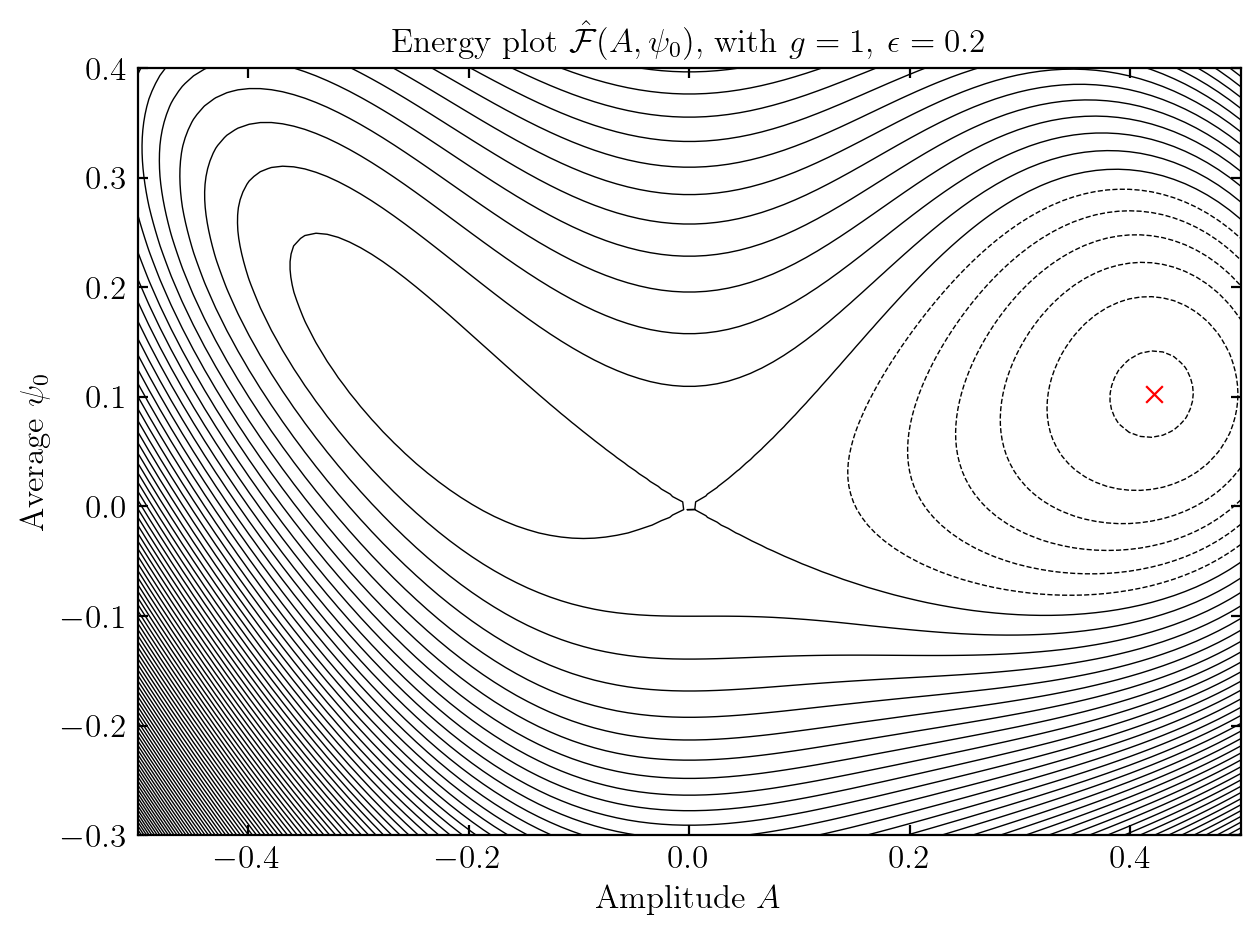
\includegraphics[width=0.5\textwidth]{imgs/weakcoupling/dipole/Energy.png}
   \caption{Two variable-energy landscape in the generalized SH model, with $g=1$ and $\varepsilon=0.2$. The red dot indicates the hexagonal state.}\label{fig:SH_Gen_Landscape}
\end{figure}
In order to test our numerical implementation, we initial a random noise around the presvisouly found average $\psi_0$ and close to the triangular state. A correct implementation should demonstrate an evolution by gradient descent of the system towards the crstyalling state. The results are illustrated in \cref{fig:SH_Gen_Noise} where we plot the average value of the order parameter, the total energy of the sytem and the $L^2$-norm of the difference between the current state and the exact solution of a hexagonal lattice $||\psi_t-\psi_{exact}||_2$ to which the system ultimately converges. The average value, even if initialized at the value corresponding to the minimum, is not kept constant throught the simulation. It drops and then raises back to stabilize around the minimum. The total energy of the system is a dreasing function in time, toward the theoretical prediction showed in dashed line. In addition, the $L^2$-norm decreases monotonically towards 0.
\begin{figure}[H]
   \centering
   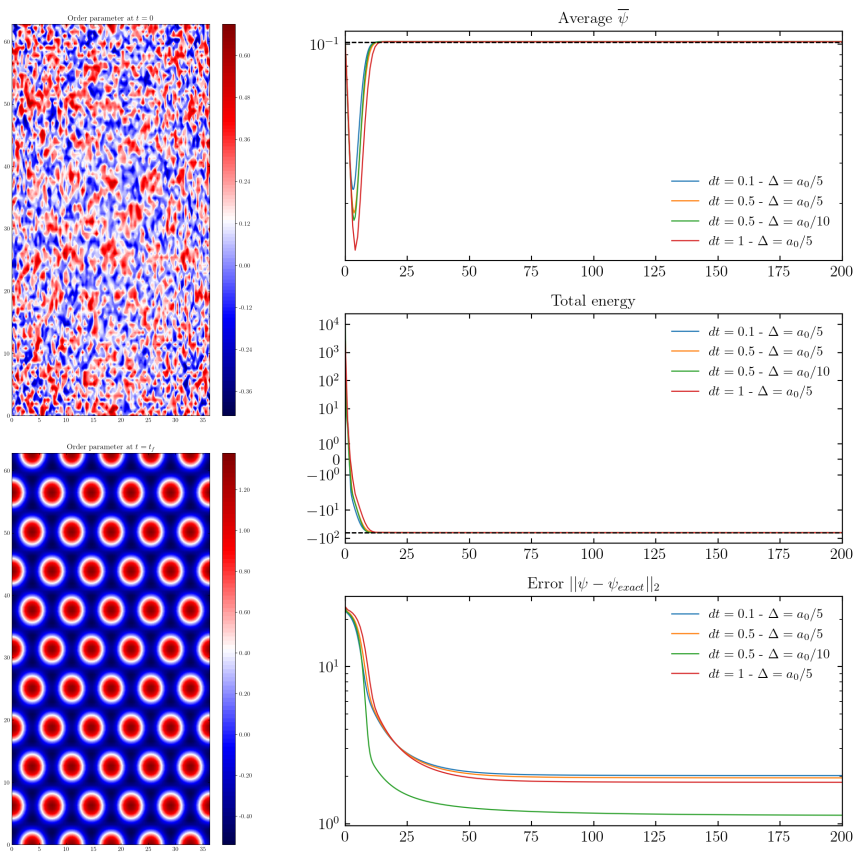
\includegraphics[width=0.77\textwidth]{imgs/weakcoupling/dipole/validationNoise.png}
   \caption{Two variable-energy landscape in the generalized SH model, with $g=1$ and $\varepsilon=0.2$. The red dot indicates the hexagonal state.}\label{fig:SH_Gen_Noise}
\end{figure}
We must highlight at this stage that we are using a generalized SH model with an additional cubic term $\psi^3$ guaranteed by picking $g \neq 0$ which differs from the classical SH/Brasovskii functional. The presence of a cubic term breaks the symmetry $\psi \longleftrightarrow -\psi$ which is a necessary condition for pattern selection to yield a crystal state within the unconserved dynamics evolution (see \cite{crossPatternFormation2009}). The cubic term can be dropped when using conserved dynamics.
\subsubsection{Localized states in the generalized model}
Even though the generalized model can showcase crytalline states with a non-conserved average, the main the limitation (i ddidn't know beforehand and i had to implement it to see that) is the possibility of developping localized stripe states within a crystal with annihilate all our topological defect paradigm. To illustrate this phenomena, we consider a perfect hexgonal lattice built using 3 resonant wave vectors exactly like we explain in the following section. In addition, we artificially seed an edge dislocation and let the system relax using the non conserved dynamics.
\begin{figure}[H]
   \centering
   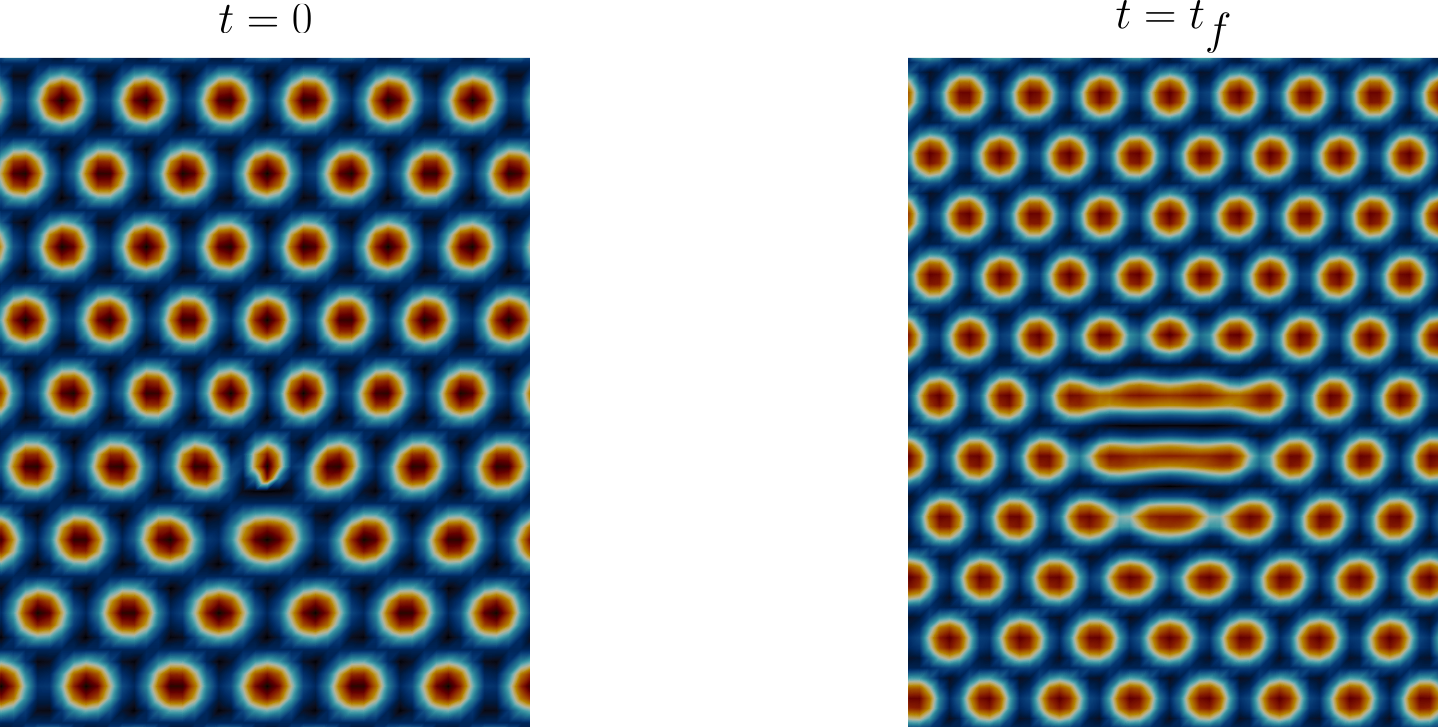
\includegraphics[width=0.77\textwidth]{imgs/weakcoupling/dipole/localization.png}
   \caption{Degeneration of seeded dislocation into a localized strip state in the generalized Swift-Hohenberg model with unconserved dynamics.}\label{fig:localization}
\end{figure}
As we illustrated in \cref{fig:localization}, the evolution of the scalar field using the non conservred dynamics degenerates into a localized strip state that evolves in time. This effects, when using a generalized SH equation, has been predicted and well studied (\cite{thieleLocalizedStatesConserved2013} \cite{burkeLocalizedStatesGeneralized2006}). Due to localized stripping, dislocation is lost and the model cannot be used to study their motion and Mechanical properties.\\


As a conclusion, we drop in the what follows and until otherwise said, the cubic term in the generalized model and work with the classical model $(g=0)$. Hence, the only way to obtain crystal state is to use a consrved dynamic evolution. The issue with this evolution equation is the presence of a sixth order spatial derivative difficult to deal with from a finite-element paradigm. Alternatives consist of using classical Lagrange multipliers to enforce average conservation or space-times dependent Lagrange multipliers (\cite{leeNewConservativeSwift2020}). Coupling phase field models with elasticity while ensuring mass conservation has been a classical question at the intersection of condensed matter physics and mechanics, a review of possible ways of coupling is presented in \cite{bartelsCahnHilliardPhase2021} \marginpar{analyze ref}. This topic was classically tackeled through coupling Cahn-Hillard with elasticity, Cahn-Hillard being the the mass-conserving version of Allen-Cahn model. (The relationship between both is the same as the one we are interested in). 
\begin{mybox}
In what follows we set $g=0$ (classical \emph{Swift-Hohenberg}). Our main issue is not mass conservation but ratehr coupling the two theories. Thus, we use a simple method to enforce mass conservation: The unconserved equation is used, keeping a fourth order pde and the scalar field is updated at each time step by adding a correction. This the step in highligheted in red in \cref{alg:UncoupledPFCFDM}.
\end{mybox}

\subsubsection{Relaxation of a stable dislocation dipole}
As a benchmark case we study the relaxation of a dislocation dipole in a 2d hexgonal lattice, as performed in \cite{upadhyayCouplingPhaseField2024}. The considered domain is a rectangular domain with sides $L=N_x dx$ and $H=N_y dy$. The grid spacing is chosen in order to have around 6 grid points around each "atom" (atoms are located at the maximums of the order parameter $\psi$ ); we chose $dx=a_0/7$, $dy=\sqrt{3}a_0/12$ where $a_0$ is the lattice parameter. Finally, we pick $N_x=602$ and $N_y=900$.\\
A hexgonal lattice is using $N=3$ wave vectors. Within the single mode approximation, we write:
\begin{equation}
   \psi(\vecc{r}) = \psi_0 +  A_0\sum_{n=1}^{2N}e^{i\vecc{q^n}\cdot \vecc r}
\end{equation}
With $\vecc{q^1}=(0,1)$, $\vecc{q^2}=(\sqrt{3}/2,-1/2)$, $\vecc{q^3}=(-\sqrt{3}/2,-1/2)$, $\vecc{q^4}=-\vecc{q^1}$,$\vecc{q^5}=-\vecc{q^2}$, $\vecc{q^6}=-\vecc{q^3}$. Minimizing the \emph{Swift-Hohenberg} energy functional yields an expression for $A_0$, \cite{elderModelingelastic2004}:
\begin{equation}
   A_0 = \frac{1}{5} \left(|\psi_0|+\frac{1}{3} \sqrt{15\varepsilon-36 \psi_0^2} \right)
\end{equation}
The phase diagram parameters $(\varepsilon,\psi_0)$ are chosen, in our case, to fall within the hexgonal lattice region: $\varepsilon=1.2$ and $\psi_0=-0.5$. Finally, we insert $p$ edge dislocations located at $(x_p,y_p)$ with a \emph{Burgers} vector $\vecc{b_p}$ by adding a shift to the phase of the scalar field $\psi$:
\begin{equation}
   \psi(\vecc{r}) = \psi_0 +  A_0\sum_{n=1}^{2N}\exp \left[ i \left(\vecc{q^n}\cdot \vecc r+ \sum_{p=1}^{2}s^{n,p} \arctan \left(\frac{y-y_p}{x-x_p}\right)\right) \right]
\end{equation}
The parameter $s^{n,p}= \frac{1}{2\pi}\vecc{q^n} \cdot \vecc{b^p}$ is the winding number. A dislocation dipole with opposite charge is intialized by setting $p=2$. The first dislocation located at $(x_1,y_1)=(L/2,3H/8)$ has a Burgers vector $\vecc{b^1}=(a_0,0)$, the second located at $(x_1,y_1)=(L/2,5H/8)$ has an opposite Burgers vector $\vecc{b^2}=(-a_0,0)$.
\begin{figure}[H]
   \centering
   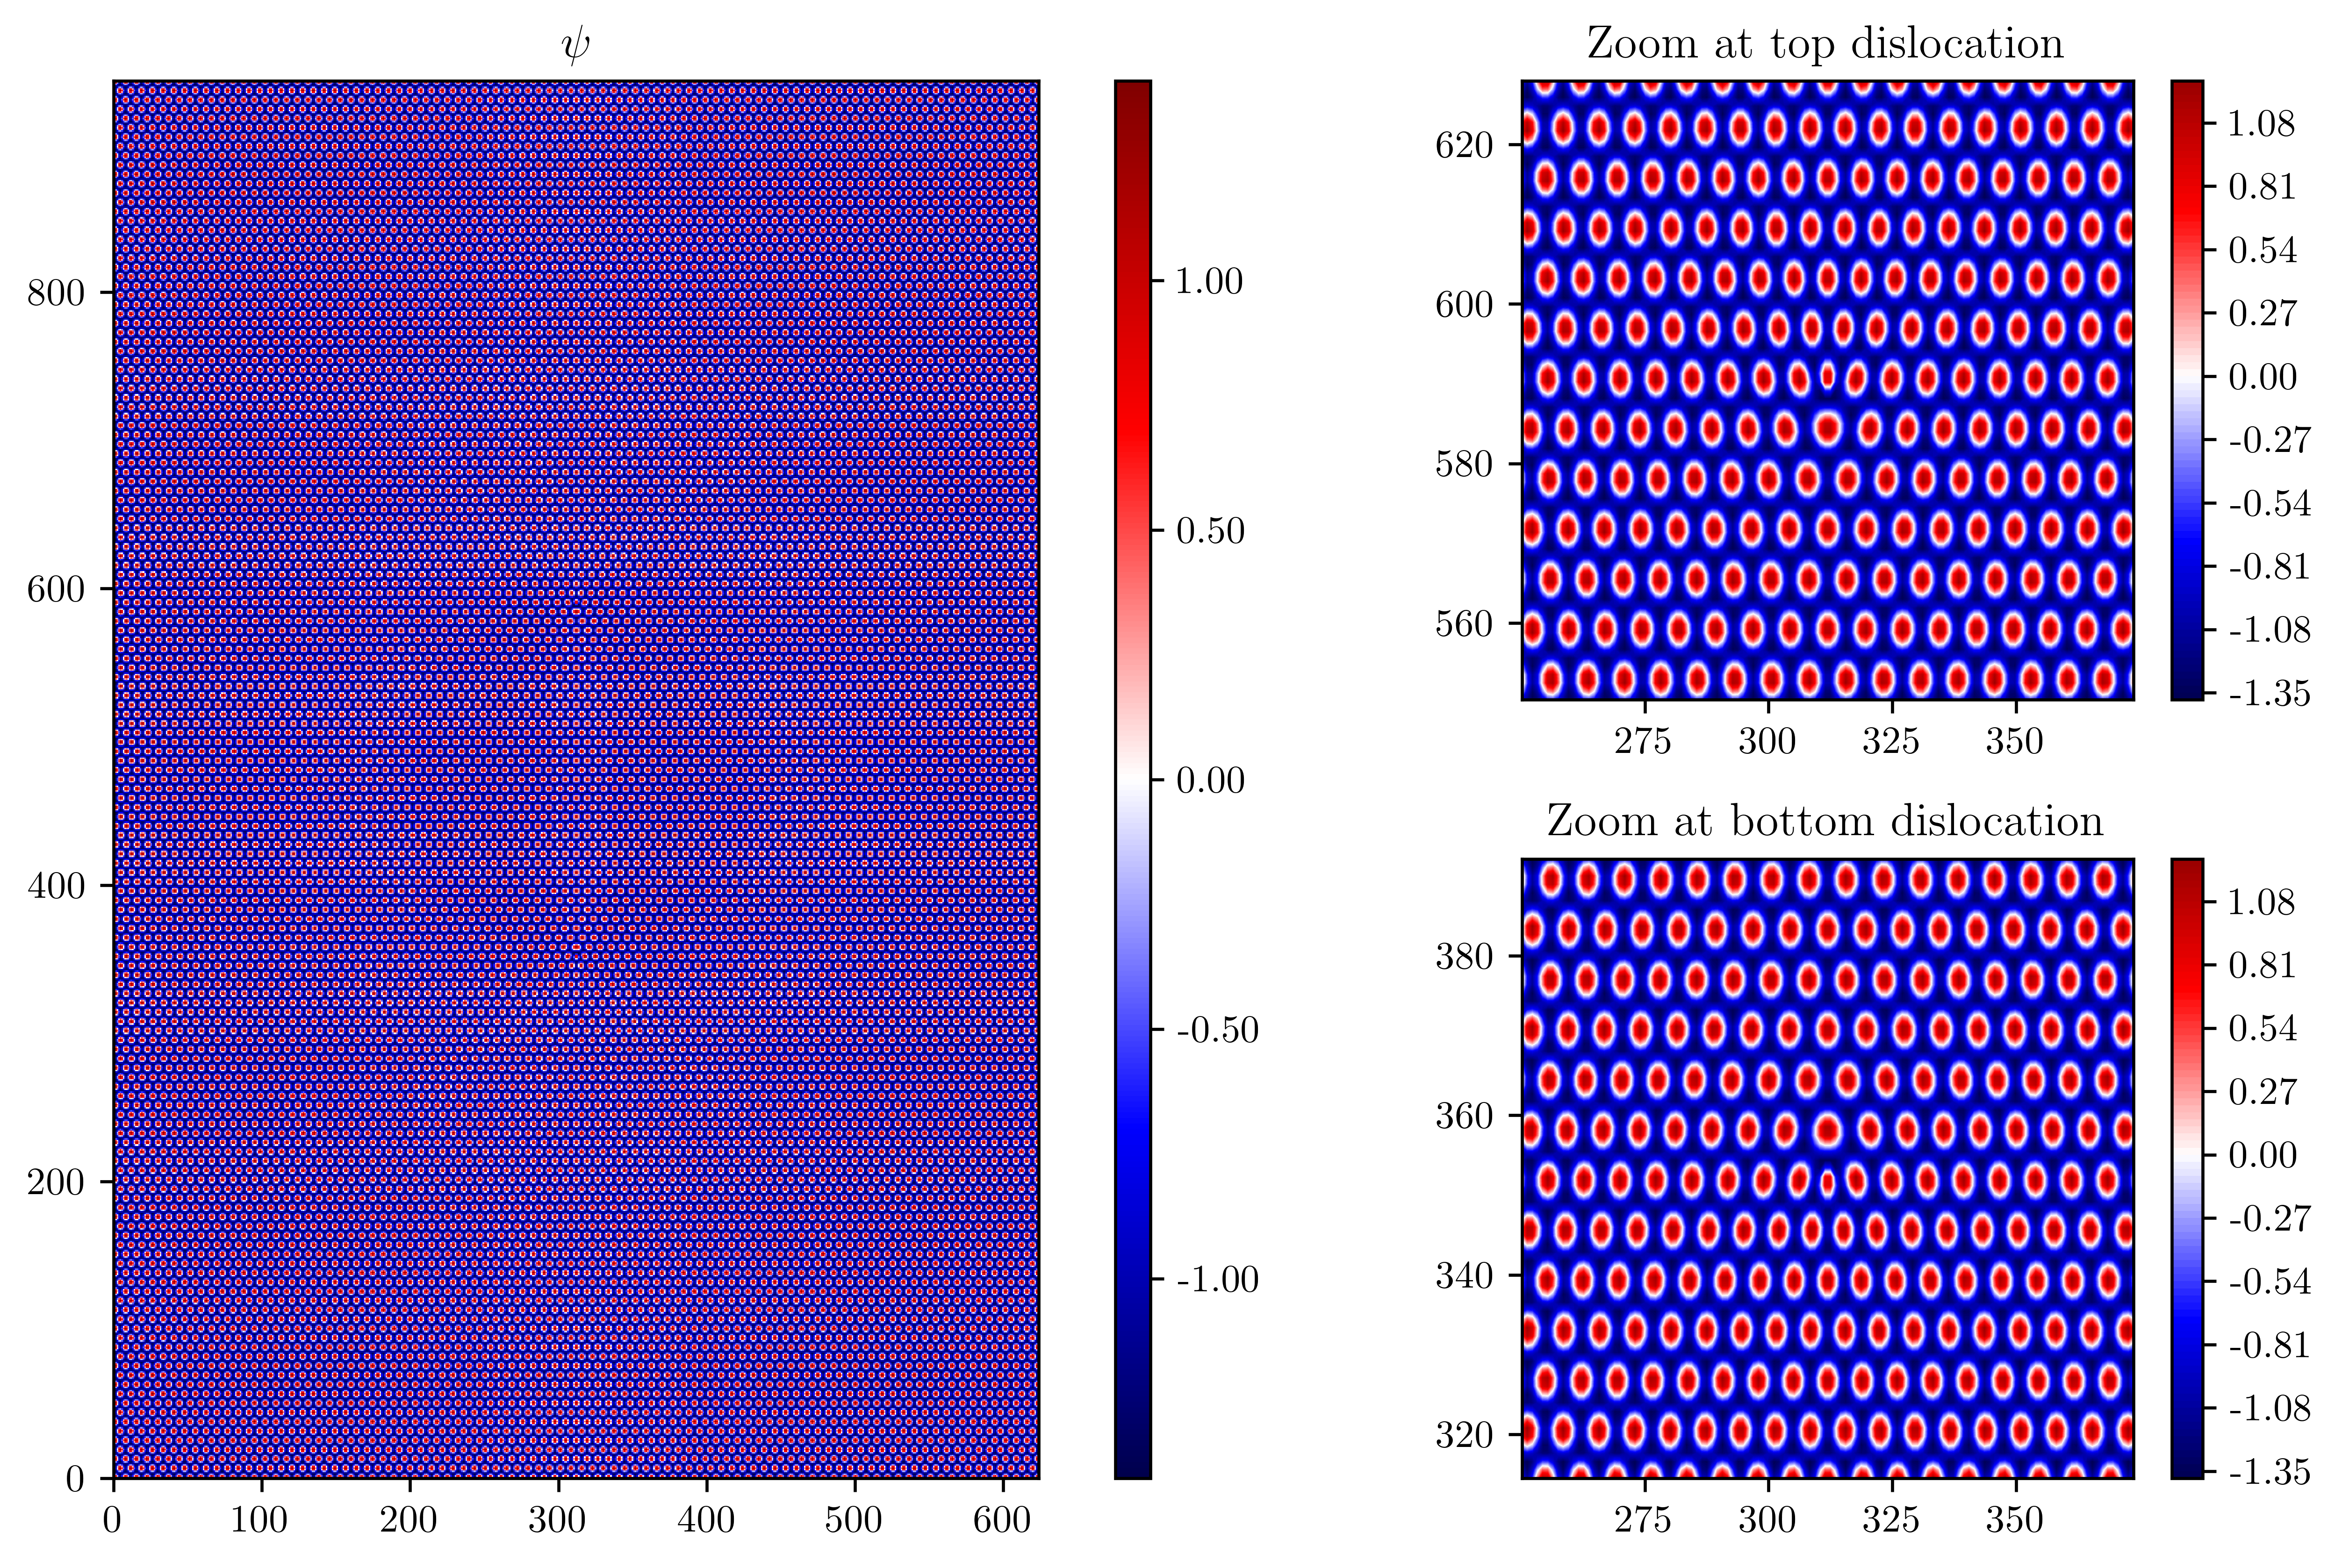
\includegraphics[width=0.9\textwidth]{imgs/weakcoupling/dipole/dipoleinit.png}
   \caption{Illustration of the initial configuration $(t=0)$ of an oppositely charged dislocation dipole. Colorbars indicate values of the order parameter $\psi$.}
\end{figure}

\end{document}

